% Options for packages loaded elsewhere
\PassOptionsToPackage{unicode}{hyperref}
\PassOptionsToPackage{hyphens}{url}
%
\documentclass[
]{article}
\usepackage{lmodern}
\usepackage{amssymb,amsmath}
\usepackage{ifxetex,ifluatex}
\ifnum 0\ifxetex 1\fi\ifluatex 1\fi=0 % if pdftex
  \usepackage[T1]{fontenc}
  \usepackage[utf8]{inputenc}
  \usepackage{textcomp} % provide euro and other symbols
\else % if luatex or xetex
  \usepackage{unicode-math}
  \defaultfontfeatures{Scale=MatchLowercase}
  \defaultfontfeatures[\rmfamily]{Ligatures=TeX,Scale=1}
\fi
% Use upquote if available, for straight quotes in verbatim environments
\IfFileExists{upquote.sty}{\usepackage{upquote}}{}
\IfFileExists{microtype.sty}{% use microtype if available
  \usepackage[]{microtype}
  \UseMicrotypeSet[protrusion]{basicmath} % disable protrusion for tt fonts
}{}
\makeatletter
\@ifundefined{KOMAClassName}{% if non-KOMA class
  \IfFileExists{parskip.sty}{%
    \usepackage{parskip}
  }{% else
    \setlength{\parindent}{0pt}
    \setlength{\parskip}{6pt plus 2pt minus 1pt}}
}{% if KOMA class
  \KOMAoptions{parskip=half}}
\makeatother
\usepackage{xcolor}
\IfFileExists{xurl.sty}{\usepackage{xurl}}{} % add URL line breaks if available
\IfFileExists{bookmark.sty}{\usepackage{bookmark}}{\usepackage{hyperref}}
\hypersetup{
  pdftitle={Lab 2},
  pdfauthor={Emilio Dorigatti},
  hidelinks,
  pdfcreator={LaTeX via pandoc}}
\urlstyle{same} % disable monospaced font for URLs
\usepackage[margin=1in]{geometry}
\usepackage{color}
\usepackage{fancyvrb}
\newcommand{\VerbBar}{|}
\newcommand{\VERB}{\Verb[commandchars=\\\{\}]}
\DefineVerbatimEnvironment{Highlighting}{Verbatim}{commandchars=\\\{\}}
% Add ',fontsize=\small' for more characters per line
\usepackage{framed}
\definecolor{shadecolor}{RGB}{248,248,248}
\newenvironment{Shaded}{\begin{snugshade}}{\end{snugshade}}
\newcommand{\AlertTok}[1]{\textcolor[rgb]{0.94,0.16,0.16}{#1}}
\newcommand{\AnnotationTok}[1]{\textcolor[rgb]{0.56,0.35,0.01}{\textbf{\textit{#1}}}}
\newcommand{\AttributeTok}[1]{\textcolor[rgb]{0.77,0.63,0.00}{#1}}
\newcommand{\BaseNTok}[1]{\textcolor[rgb]{0.00,0.00,0.81}{#1}}
\newcommand{\BuiltInTok}[1]{#1}
\newcommand{\CharTok}[1]{\textcolor[rgb]{0.31,0.60,0.02}{#1}}
\newcommand{\CommentTok}[1]{\textcolor[rgb]{0.56,0.35,0.01}{\textit{#1}}}
\newcommand{\CommentVarTok}[1]{\textcolor[rgb]{0.56,0.35,0.01}{\textbf{\textit{#1}}}}
\newcommand{\ConstantTok}[1]{\textcolor[rgb]{0.00,0.00,0.00}{#1}}
\newcommand{\ControlFlowTok}[1]{\textcolor[rgb]{0.13,0.29,0.53}{\textbf{#1}}}
\newcommand{\DataTypeTok}[1]{\textcolor[rgb]{0.13,0.29,0.53}{#1}}
\newcommand{\DecValTok}[1]{\textcolor[rgb]{0.00,0.00,0.81}{#1}}
\newcommand{\DocumentationTok}[1]{\textcolor[rgb]{0.56,0.35,0.01}{\textbf{\textit{#1}}}}
\newcommand{\ErrorTok}[1]{\textcolor[rgb]{0.64,0.00,0.00}{\textbf{#1}}}
\newcommand{\ExtensionTok}[1]{#1}
\newcommand{\FloatTok}[1]{\textcolor[rgb]{0.00,0.00,0.81}{#1}}
\newcommand{\FunctionTok}[1]{\textcolor[rgb]{0.00,0.00,0.00}{#1}}
\newcommand{\ImportTok}[1]{#1}
\newcommand{\InformationTok}[1]{\textcolor[rgb]{0.56,0.35,0.01}{\textbf{\textit{#1}}}}
\newcommand{\KeywordTok}[1]{\textcolor[rgb]{0.13,0.29,0.53}{\textbf{#1}}}
\newcommand{\NormalTok}[1]{#1}
\newcommand{\OperatorTok}[1]{\textcolor[rgb]{0.81,0.36,0.00}{\textbf{#1}}}
\newcommand{\OtherTok}[1]{\textcolor[rgb]{0.56,0.35,0.01}{#1}}
\newcommand{\PreprocessorTok}[1]{\textcolor[rgb]{0.56,0.35,0.01}{\textit{#1}}}
\newcommand{\RegionMarkerTok}[1]{#1}
\newcommand{\SpecialCharTok}[1]{\textcolor[rgb]{0.00,0.00,0.00}{#1}}
\newcommand{\SpecialStringTok}[1]{\textcolor[rgb]{0.31,0.60,0.02}{#1}}
\newcommand{\StringTok}[1]{\textcolor[rgb]{0.31,0.60,0.02}{#1}}
\newcommand{\VariableTok}[1]{\textcolor[rgb]{0.00,0.00,0.00}{#1}}
\newcommand{\VerbatimStringTok}[1]{\textcolor[rgb]{0.31,0.60,0.02}{#1}}
\newcommand{\WarningTok}[1]{\textcolor[rgb]{0.56,0.35,0.01}{\textbf{\textit{#1}}}}
\usepackage{graphicx}
\makeatletter
\def\maxwidth{\ifdim\Gin@nat@width>\linewidth\linewidth\else\Gin@nat@width\fi}
\def\maxheight{\ifdim\Gin@nat@height>\textheight\textheight\else\Gin@nat@height\fi}
\makeatother
% Scale images if necessary, so that they will not overflow the page
% margins by default, and it is still possible to overwrite the defaults
% using explicit options in \includegraphics[width, height, ...]{}
\setkeys{Gin}{width=\maxwidth,height=\maxheight,keepaspectratio}
% Set default figure placement to htbp
\makeatletter
\def\fps@figure{htbp}
\makeatother
\setlength{\emergencystretch}{3em} % prevent overfull lines
\providecommand{\tightlist}{%
  \setlength{\itemsep}{0pt}\setlength{\parskip}{0pt}}
\setcounter{secnumdepth}{-\maxdimen} % remove section numbering
\ifluatex
  \usepackage{selnolig}  % disable illegal ligatures
\fi

\title{Lab 2}
\author{Emilio Dorigatti}
\date{2020-11-13}

\begin{document}
\maketitle

\hypertarget{exercise-1}{%
\subsection{Exercise 1}\label{exercise-1}}

Consider a neural network with one hidden layer with threshold
activation function (i.e., \(\tau(x)=\mathbf{1}[x>0]\)) and one output
neuron with no activation function. Prove that such a neural network
cannot \emph{exactly} separate the cyan (\(y=1\)) and white (\(y=0\))
areas in Figure 1.

\begin{figure}
\centering

\includegraphics[width=2.60417in,height=\textheight]{lab2f1.png}
\caption{A region that cannot be classified correctly by a neural
network with a single hidden layer.}
\end{figure}

\textbf{Hint}: start by assuming that such a neural network exists and
has two neurons in the hidden layer. Consider four points, one for each
of the four regions, \(\textbf{x}_1,\ldots,\textbf{x}_4\) with
\(y_2=y_4=0\) and \(y_1=y_3=1\). Compute the difference between the
predictions of points with different labels,
\(g(\textbf{x}_1)-g(\textbf{x}_2)\) and
\(g(\textbf{x}_4)-g(\textbf{x}_3)\). You should reach a contradiction,
meaning that such a neural network does not exists.

\hypertarget{solution}{%
\subsubsection{Solution}\label{solution}}

Assume that such a neural network exists. Then, it computes a function
\(g\) of the form:

\[
g(\textbf{x})=\sum_{i=1}^m w_i\cdot \tau(\textbf{x}^T\textbf{v}_i+c_i)+b
\]

Now consider four points as in Figure 2, so that
\(g(\textbf{x}_1)=g(\textbf{x}_3)=1\) and
\(g(\textbf{x}_2)=g(\textbf{x}_4)=0\). Moreover, assume that the first
hidden neuron models \(L_1\), so that it has a positive activation for
\(\textbf{x}_2\) and \(\textbf{x}_3\), and zero for \(\textbf{x}_1\) and
\(\textbf{x}_4\).

\begin{figure}
\centering
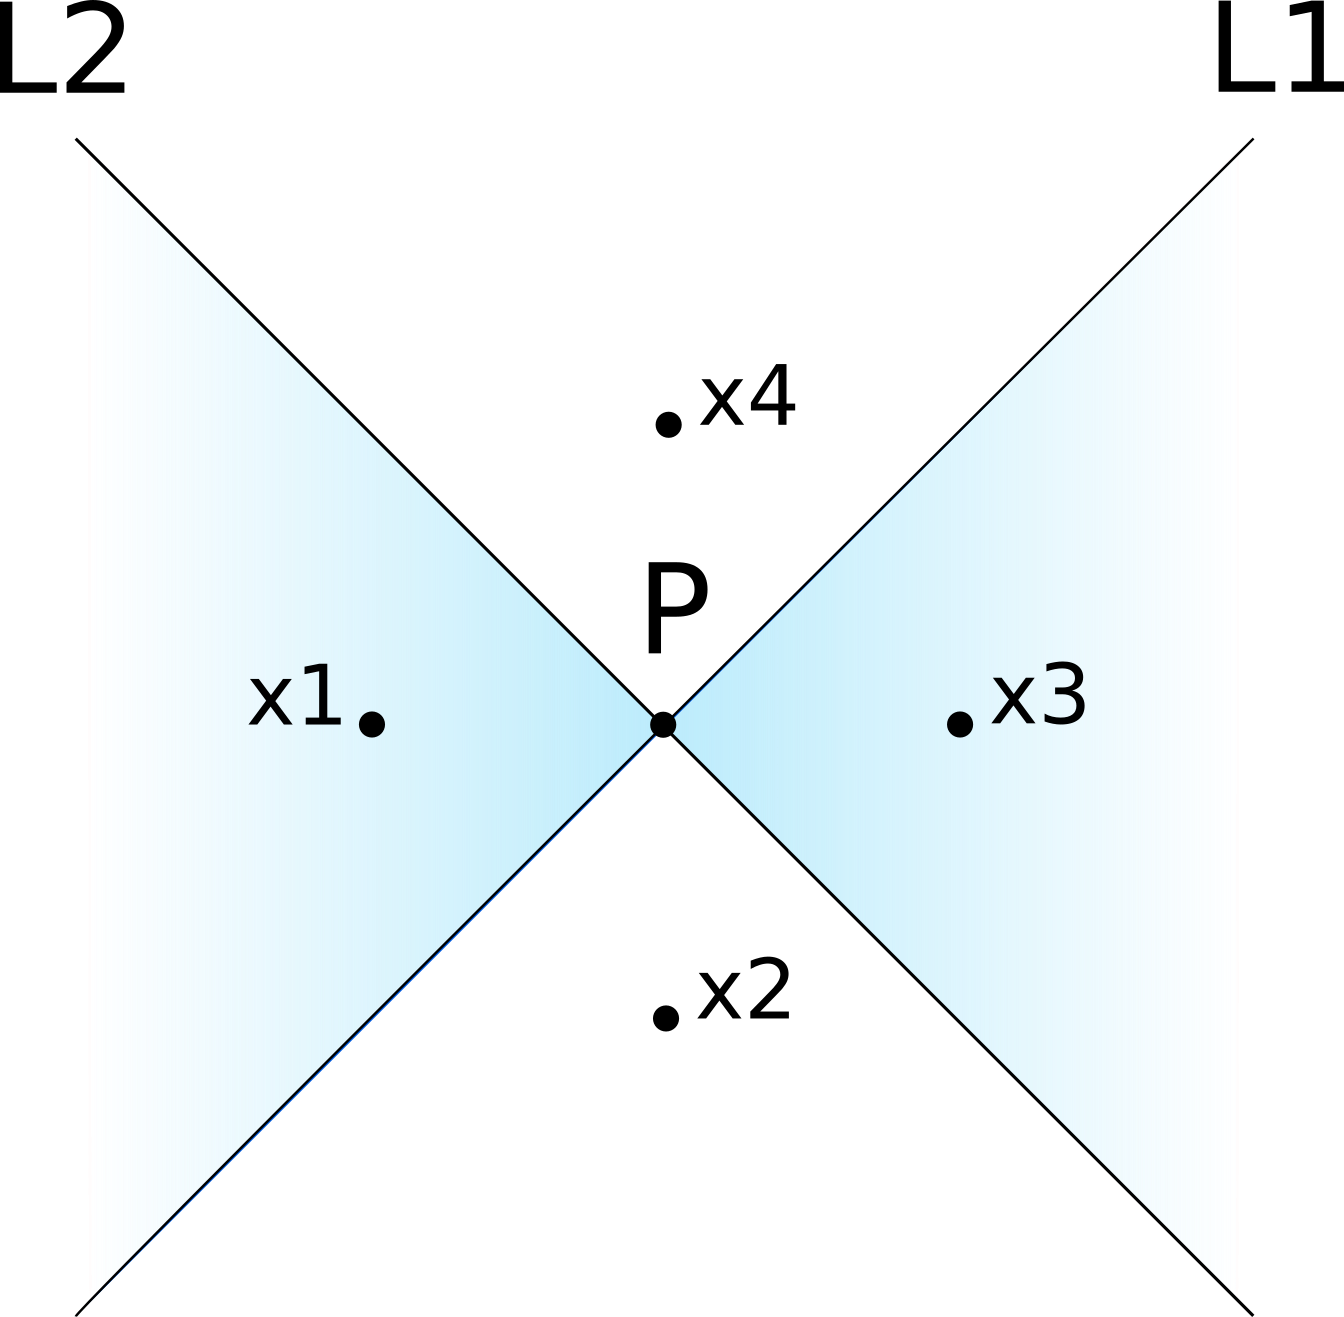
\includegraphics[width=2.60417in,height=\textheight]{lab2f2.png}
\caption{Four points in the four regions.}
\end{figure}

The difference between the predictions for \(\textbf{x}_1\) and
\(\textbf{x}_2\) is

\begin{align*}
g(\textbf{x}_1)-g(\textbf{x}_2)
&= \sum_{i=1}^m w_i\cdot \tau(\textbf{x}_1^T\textbf{v}_i+c_i)+b-\sum_{i=1}^m w_i\cdot \tau(\textbf{x}_2^T\textbf{v}_i+c_i)-b \\
&= w_1\cdot \tau(\textbf{x}_1^T\textbf{v}_1+c_1)-w_1\cdot \tau(\textbf{x}_2^T\textbf{v}_1+c_1) \\
& =w_1\cdot 0-w_1\cdot 1 \\
&= -w_1 = 1
\end{align*}

The second step follows because when going from \(\textbf{x}_1\) to
\(\textbf{x}_2\) we only cross \(L_1\), and we stay on the same side of
every other line. The last step follows because we know that
\(g(\textbf{x}_1)=1\) and that \(g(\textbf{x}_2)=0\). This allows us to
conclude that \(w_1=-1\).

The same reasoning applies to \(\textbf{x}_4\) and \(\textbf{x}_3\),
too:

\begin{align*}
g(\textbf{x}_4)-g(\textbf{x}_3)
&=w_1\cdot \tau(\textbf{x}_4^T\textbf{v}_1+c_1)-w_1\cdot \tau(\textbf{x}_3^T\textbf{v}_1+c_1)) \\
&=-w_1 =-1
\end{align*}

Which implies that \(w_1=1\). This contradicts what we found previously,
hence no such neural network exists.

Note: this proof is presented in

Blum, Edward K., and Leong Kwan Li. 1991. ``Approximation Theory and
Feedforward Networks.'' \emph{Neural Networks} (4): 511--15.
\url{https://doi.org/10.1016/0893-6080(91)90047-9.7}

\hypertarget{exercise-2}{%
\subsection{Exercise 2}\label{exercise-2}}

In this exercise, we are going to create a neural network with two
hidden layers and threshold activation that can correctly separate the
cyan region from the rest in the plot below. We will do this by
composing linear classifiers just like we did in the previous lab.

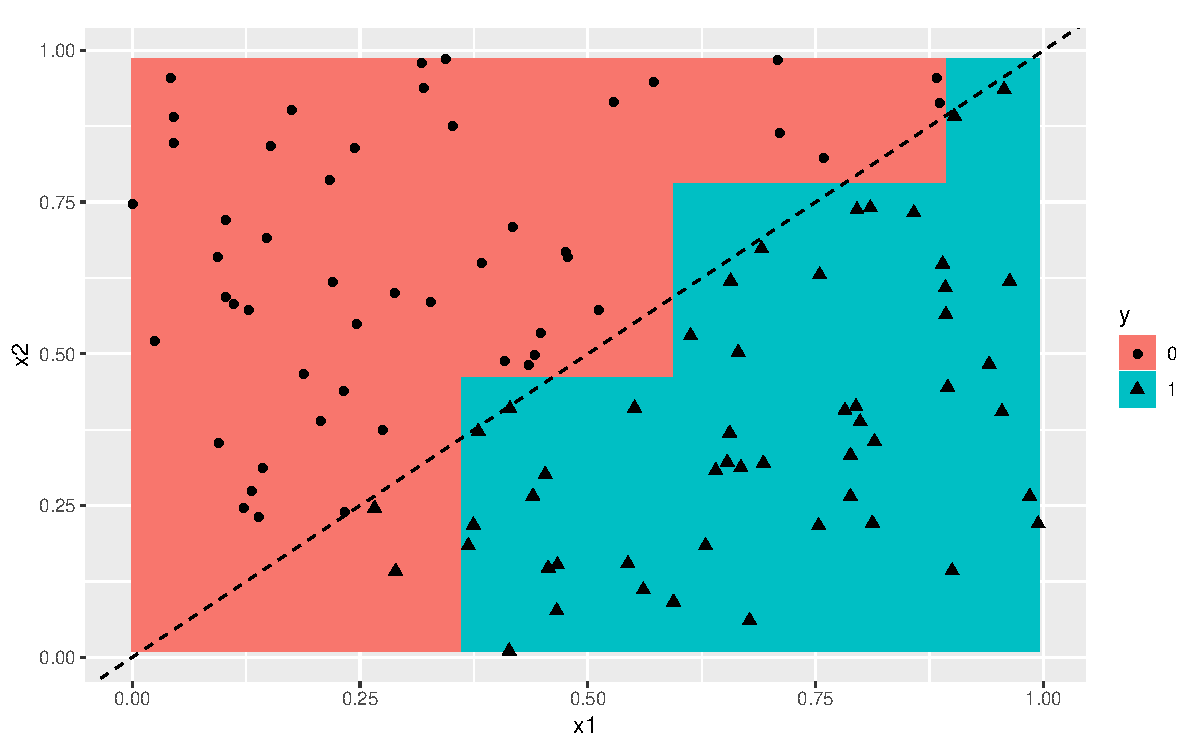
\includegraphics{lab2-solutions_files/figure-latex/unnamed-chunk-1-1.pdf}

Let us create a dataset containing points on a grid to test the network:

\begin{Shaded}
\begin{Highlighting}[]
\CommentTok{\# build a grid of equally{-}spaced points, plus a column for the bias}
\NormalTok{data }\OtherTok{=} \FunctionTok{as.matrix}\NormalTok{(}\FunctionTok{expand.grid}\NormalTok{(}
  \AttributeTok{x0 =} \DecValTok{1}\SpecialCharTok{:}\DecValTok{1}\NormalTok{,}
  \AttributeTok{x1 =} \FunctionTok{seq}\NormalTok{(}\SpecialCharTok{{-}}\DecValTok{2}\NormalTok{, }\DecValTok{2}\NormalTok{, }\DecValTok{1} \SpecialCharTok{/} \DecValTok{25}\NormalTok{),}
  \AttributeTok{x2 =} \FunctionTok{seq}\NormalTok{(}\SpecialCharTok{{-}}\DecValTok{2}\NormalTok{, }\DecValTok{2}\NormalTok{, }\DecValTok{1} \SpecialCharTok{/} \DecValTok{25}\NormalTok{)}
\NormalTok{))}

\FunctionTok{head}\NormalTok{(data)}
\end{Highlighting}
\end{Shaded}

\begin{verbatim}
##      x0    x1 x2
## [1,]  1 -2.00 -2
## [2,]  1 -1.96 -2
## [3,]  1 -1.92 -2
## [4,]  1 -1.88 -2
## [5,]  1 -1.84 -2
## [6,]  1 -1.80 -2
\end{verbatim}

\hypertarget{first-hidden-layer}{%
\subsubsection{First hidden layer}\label{first-hidden-layer}}

The first hidden layer contains four neurons, each of which corresponds
to a line in the plot below:

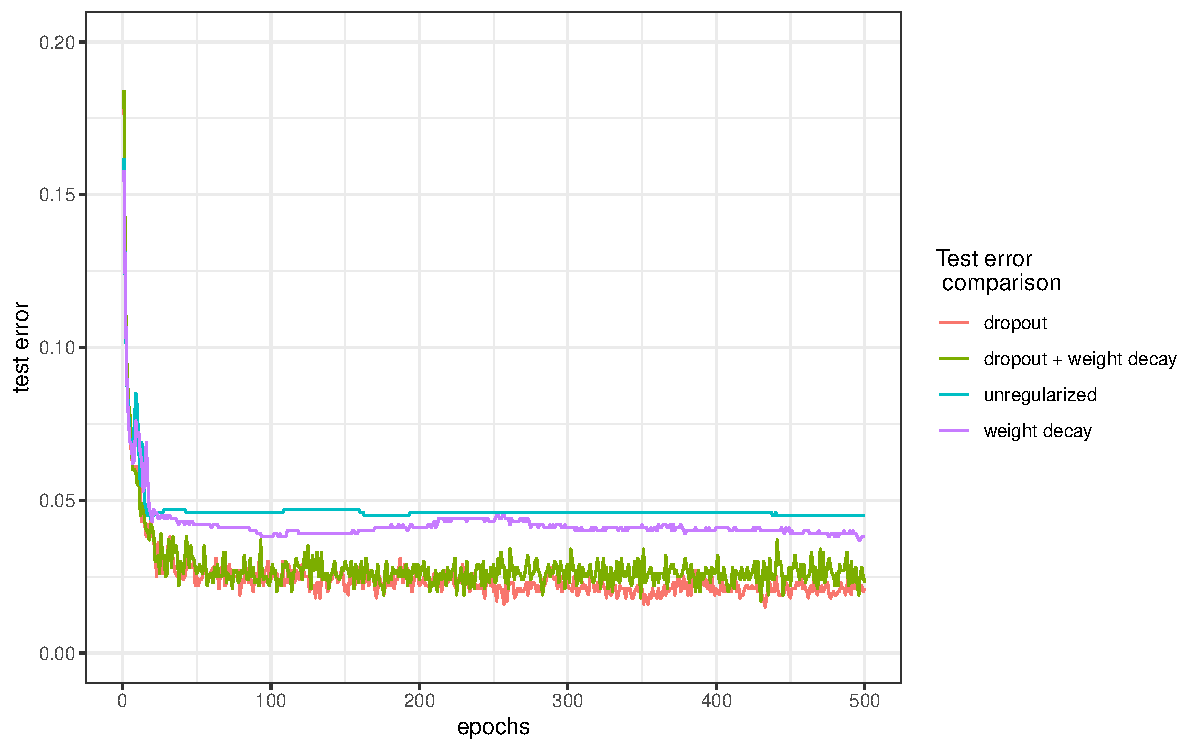
\includegraphics{lab2-solutions_files/figure-latex/unnamed-chunk-3-1.pdf}

The following functions visualizes the decision boundary of a neuron
with sigmoid activation, \(y=\sigma(a+bx_1+cx_2)\). You can use it to
help you find the right values for the weights.

\begin{Shaded}
\begin{Highlighting}[]
\FunctionTok{library}\NormalTok{(scales)}

\NormalTok{plot\_grid }\OtherTok{=} \ControlFlowTok{function}\NormalTok{(predictions) \{}
  \CommentTok{\# plots the predicted value for each point on the grid;}
  \CommentTok{\# the predictions should have one column and}
  \CommentTok{\# the same number of rows (10,201) as the data}
\NormalTok{  df }\OtherTok{=} \FunctionTok{cbind}\NormalTok{(}\FunctionTok{as.data.frame}\NormalTok{(data), }\AttributeTok{y =}\NormalTok{ predictions)}
  \FunctionTok{ggplot}\NormalTok{() }\SpecialCharTok{+}
    \FunctionTok{geom\_tile}\NormalTok{(}\FunctionTok{aes}\NormalTok{(}\AttributeTok{x =}\NormalTok{ x1, }\AttributeTok{y =}\NormalTok{ x2, }\AttributeTok{fill =}\NormalTok{ y, }\AttributeTok{color =}\NormalTok{ y), df) }\SpecialCharTok{+}
    \FunctionTok{scale\_color\_gradient2}\NormalTok{(}\AttributeTok{low =} \FunctionTok{muted}\NormalTok{(}\StringTok{"blue"}\NormalTok{, }\DecValTok{70}\NormalTok{), }\AttributeTok{mid =} \StringTok{"white"}\NormalTok{,}
                         \AttributeTok{high =} \FunctionTok{muted}\NormalTok{(}\StringTok{"red"}\NormalTok{, }\DecValTok{70}\NormalTok{), }\AttributeTok{limits =} \FunctionTok{c}\NormalTok{(}\DecValTok{0}\NormalTok{, }\DecValTok{1}\NormalTok{),}
                         \AttributeTok{midpoint =} \FloatTok{0.5}\NormalTok{) }\SpecialCharTok{+}
    \FunctionTok{scale\_fill\_gradient2}\NormalTok{(}\AttributeTok{low =} \FunctionTok{muted}\NormalTok{(}\StringTok{"blue"}\NormalTok{, }\DecValTok{70}\NormalTok{), }\AttributeTok{mid =} \StringTok{"white"}\NormalTok{,}
                        \AttributeTok{high =} \FunctionTok{muted}\NormalTok{(}\StringTok{"red"}\NormalTok{, }\DecValTok{70}\NormalTok{), }\AttributeTok{limits =} \FunctionTok{c}\NormalTok{(}\DecValTok{0}\NormalTok{, }\DecValTok{1}\NormalTok{),}
                        \AttributeTok{midpoint =} \FloatTok{0.5}\NormalTok{) }\SpecialCharTok{+}
    \FunctionTok{geom\_line}\NormalTok{(}\FunctionTok{aes}\NormalTok{(}\AttributeTok{x =} \FunctionTok{c}\NormalTok{(}\SpecialCharTok{{-}}\FloatTok{1.25}\NormalTok{, }\FloatTok{1.25}\NormalTok{), }\AttributeTok{y =} \FunctionTok{c}\NormalTok{(}\FloatTok{1.25}\NormalTok{, }\SpecialCharTok{{-}}\FloatTok{1.25}\NormalTok{)), }\AttributeTok{inherit.aes =}\NormalTok{ F) }\SpecialCharTok{+}
    \FunctionTok{geom\_line}\NormalTok{(}\FunctionTok{aes}\NormalTok{(}\AttributeTok{x =} \FunctionTok{c}\NormalTok{(}\SpecialCharTok{{-}}\FloatTok{1.25}\NormalTok{, }\FloatTok{1.25}\NormalTok{), }\AttributeTok{y =} \FunctionTok{c}\NormalTok{(}\SpecialCharTok{{-}}\FloatTok{1.25}\NormalTok{, }\FloatTok{1.25}\NormalTok{)), }\AttributeTok{inherit.aes =}\NormalTok{ F) }\SpecialCharTok{+}
    \FunctionTok{geom\_line}\NormalTok{(}\FunctionTok{aes}\NormalTok{(}\AttributeTok{x =} \FunctionTok{c}\NormalTok{(}\SpecialCharTok{{-}}\DecValTok{1}\NormalTok{, }\SpecialCharTok{{-}}\DecValTok{1}\NormalTok{), }\AttributeTok{y =} \FunctionTok{c}\NormalTok{(}\SpecialCharTok{{-}}\FloatTok{1.5}\NormalTok{, }\FloatTok{1.5}\NormalTok{)), }\AttributeTok{inherit.aes =}\NormalTok{ F) }\SpecialCharTok{+}
    \FunctionTok{geom\_line}\NormalTok{(}\FunctionTok{aes}\NormalTok{(}\AttributeTok{x =} \FunctionTok{c}\NormalTok{(}\DecValTok{1}\NormalTok{, }\DecValTok{1}\NormalTok{), }\AttributeTok{y =} \FunctionTok{c}\NormalTok{(}\SpecialCharTok{{-}}\FloatTok{1.5}\NormalTok{, }\FloatTok{1.5}\NormalTok{)), }\AttributeTok{inherit.aes =}\NormalTok{ F)}
\NormalTok{\}}

\NormalTok{activation }\OtherTok{=} \ControlFlowTok{function}\NormalTok{(x) \{}
  \FunctionTok{ifelse}\NormalTok{(x }\SpecialCharTok{\textgreater{}} \DecValTok{0}\NormalTok{, }\DecValTok{1}\NormalTok{, }\DecValTok{0}\NormalTok{)}
\NormalTok{\}}

\NormalTok{plot\_decision\_boundary\_first\_hidden }\OtherTok{=} \ControlFlowTok{function}\NormalTok{(a, b, c) \{}
\NormalTok{  neuron\_output }\OtherTok{=}\NormalTok{ (}
    \FunctionTok{activation}\NormalTok{(data }\SpecialCharTok{\%*\%} \FunctionTok{c}\NormalTok{(a, b, c))}
\NormalTok{  );}
  \FunctionTok{plot\_grid}\NormalTok{(neuron\_output);}
\NormalTok{\}}

\FunctionTok{plot\_decision\_boundary\_first\_hidden}\NormalTok{(}\DecValTok{1}\NormalTok{, }\SpecialCharTok{{-}}\DecValTok{2}\NormalTok{, }\DecValTok{1}\NormalTok{)}
\end{Highlighting}
\end{Shaded}

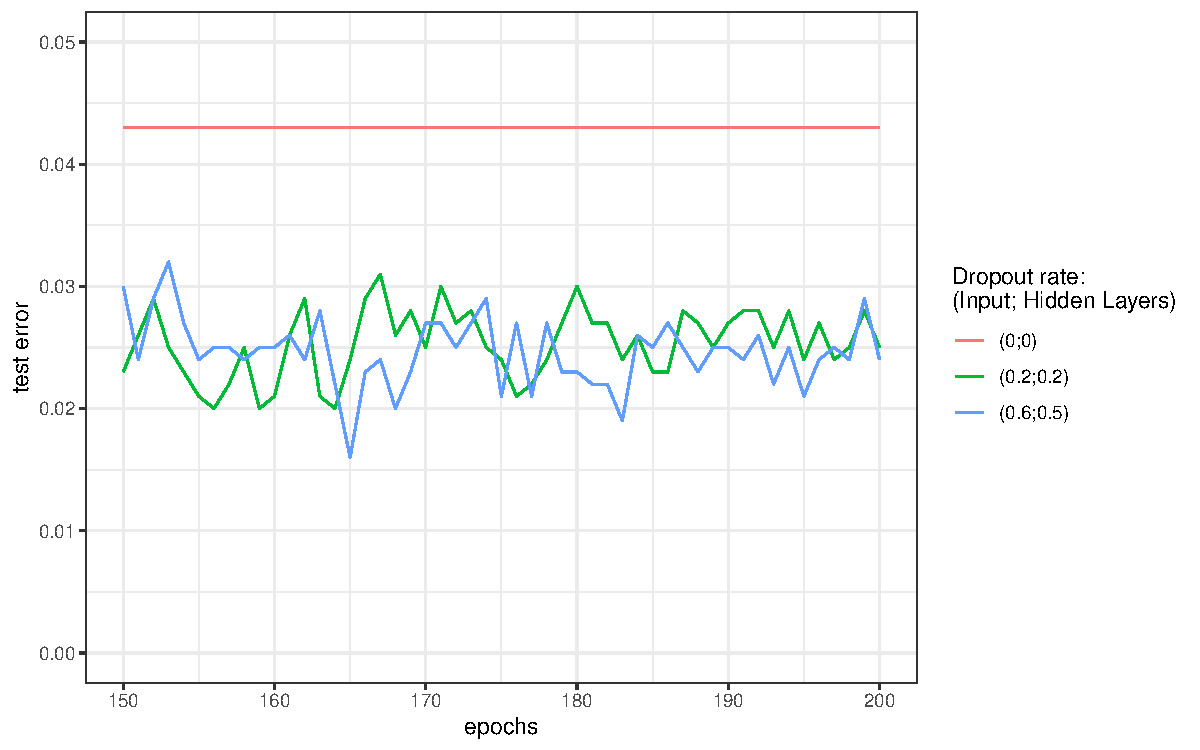
\includegraphics{lab2-solutions_files/figure-latex/unnamed-chunk-4-1.pdf}

For convenience, we group the parameters of the four neurons into a
matrix with three rows and five columns (one is for the bias), so that
their output can be computed in a single matrix multiplication. Each
column contains the weights of a different neuron. The first column
contains a ``fake'' hidden neuron for the bias, whose value is always
one. Note that the first row of the weight matrix is connected to the
bias of the previous layer.

\begin{Shaded}
\begin{Highlighting}[]
\NormalTok{weights1 }\OtherTok{=} \FunctionTok{matrix}\NormalTok{(}\FunctionTok{c}\NormalTok{(}
  \DecValTok{1}\NormalTok{, }\DecValTok{0}\NormalTok{, }\DecValTok{0}\NormalTok{,   }\CommentTok{\# bias neuron connected to the bias of the inputs}
  \DecValTok{1}\NormalTok{, }\SpecialCharTok{{-}}\DecValTok{1}\NormalTok{, }\DecValTok{0}\NormalTok{,}
  \DecValTok{1}\NormalTok{, }\DecValTok{1}\NormalTok{, }\DecValTok{0}\NormalTok{,}
  \DecValTok{0}\NormalTok{, }\DecValTok{1}\NormalTok{, }\SpecialCharTok{{-}}\DecValTok{1}\NormalTok{,}
  \DecValTok{0}\NormalTok{, }\DecValTok{1}\NormalTok{, }\DecValTok{1}
\NormalTok{), }\AttributeTok{ncol =} \DecValTok{5}\NormalTok{);}

\FunctionTok{dim}\NormalTok{(weights1)}
\end{Highlighting}
\end{Shaded}

\begin{verbatim}
## [1] 3 5
\end{verbatim}

Let us plot the predictions of the four neurons:

\begin{Shaded}
\begin{Highlighting}[]
\CommentTok{\# make sure that the decision boundary of the neurons corresponds to the four lines}
\FunctionTok{plot\_decision\_boundary\_first\_hidden}\NormalTok{(weights1[}\DecValTok{1}\NormalTok{, }\DecValTok{2}\NormalTok{], weights1[}\DecValTok{2}\NormalTok{, }\DecValTok{2}\NormalTok{], weights1[}\DecValTok{3}\NormalTok{, }\DecValTok{2}\NormalTok{]);}
\end{Highlighting}
\end{Shaded}

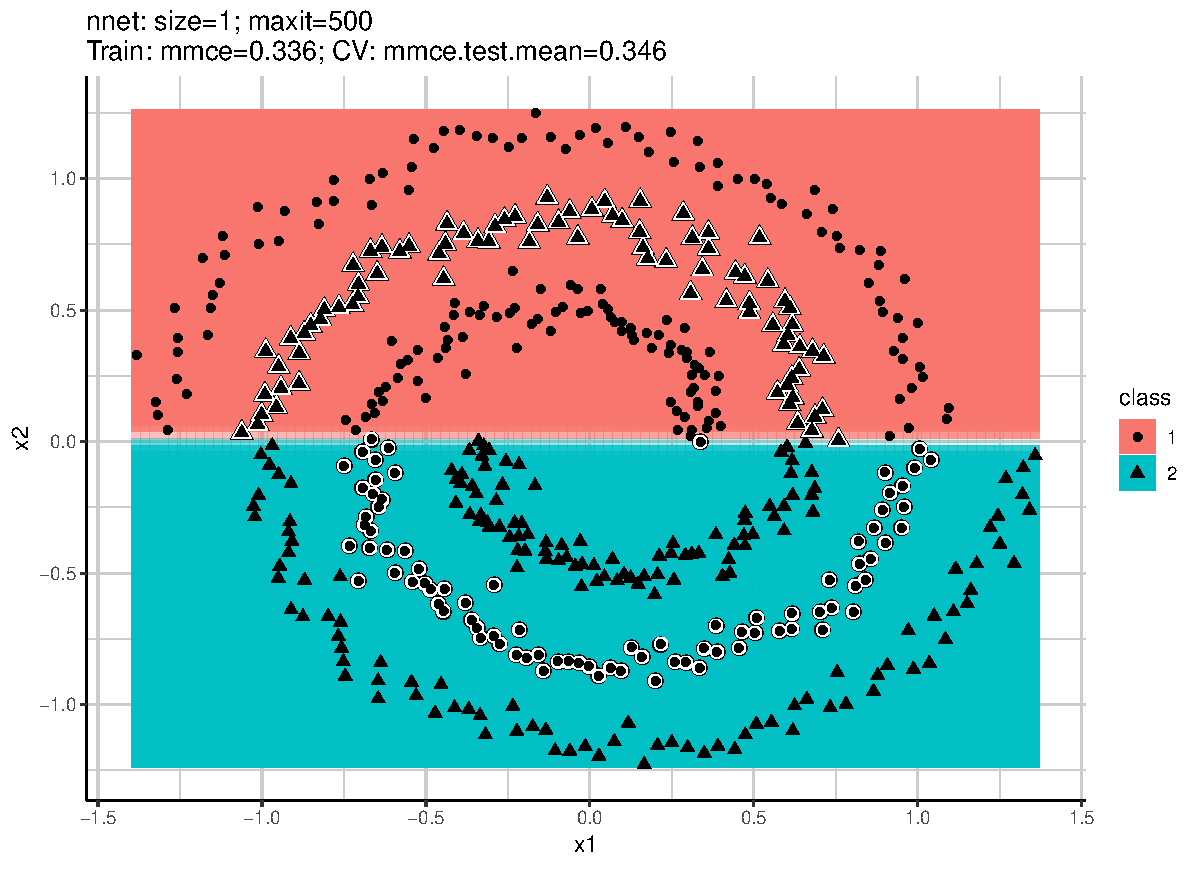
\includegraphics{lab2-solutions_files/figure-latex/unnamed-chunk-6-1.pdf}

\begin{Shaded}
\begin{Highlighting}[]
\FunctionTok{plot\_decision\_boundary\_first\_hidden}\NormalTok{(weights1[}\DecValTok{1}\NormalTok{, }\DecValTok{3}\NormalTok{], weights1[}\DecValTok{2}\NormalTok{, }\DecValTok{3}\NormalTok{], weights1[}\DecValTok{3}\NormalTok{, }\DecValTok{3}\NormalTok{]);}
\end{Highlighting}
\end{Shaded}

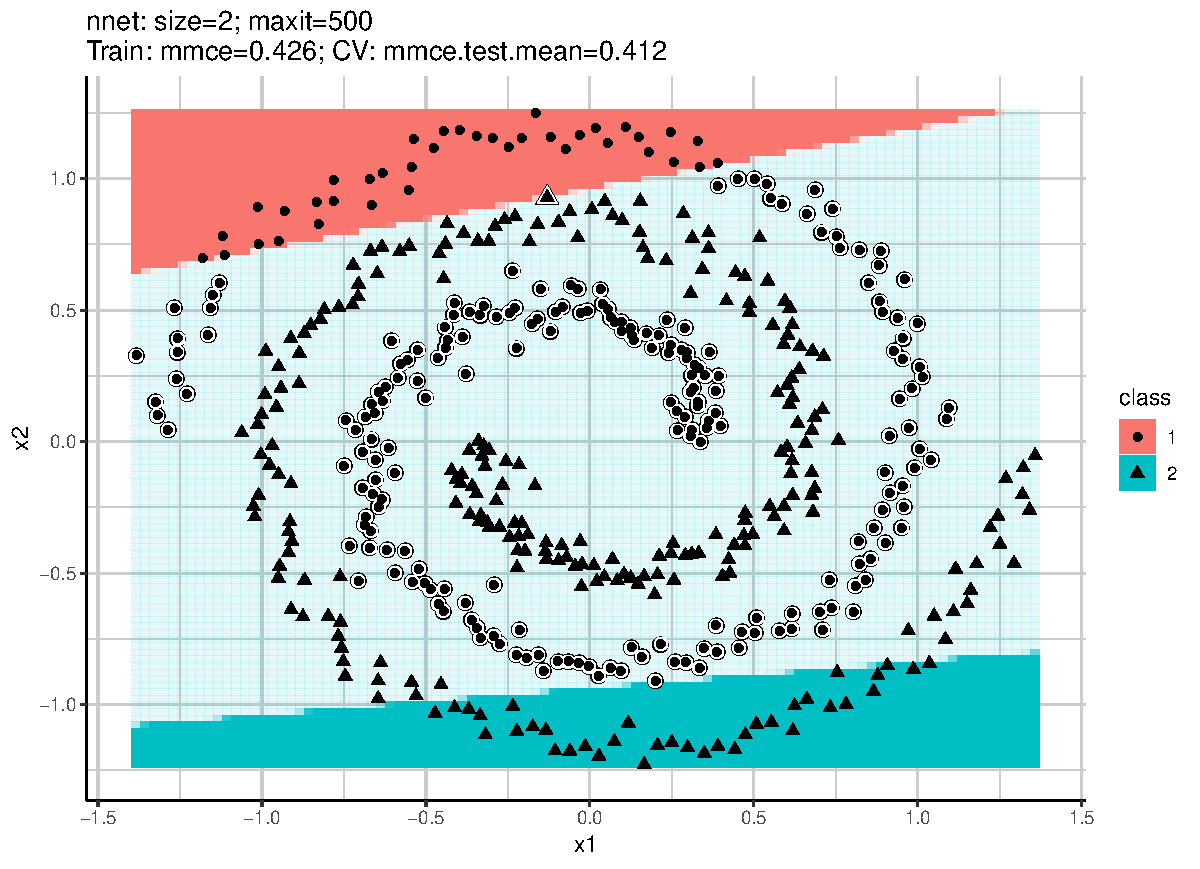
\includegraphics{lab2-solutions_files/figure-latex/unnamed-chunk-6-2.pdf}

\begin{Shaded}
\begin{Highlighting}[]
\FunctionTok{plot\_decision\_boundary\_first\_hidden}\NormalTok{(weights1[}\DecValTok{1}\NormalTok{, }\DecValTok{4}\NormalTok{], weights1[}\DecValTok{2}\NormalTok{, }\DecValTok{4}\NormalTok{], weights1[}\DecValTok{3}\NormalTok{, }\DecValTok{4}\NormalTok{]);}
\end{Highlighting}
\end{Shaded}

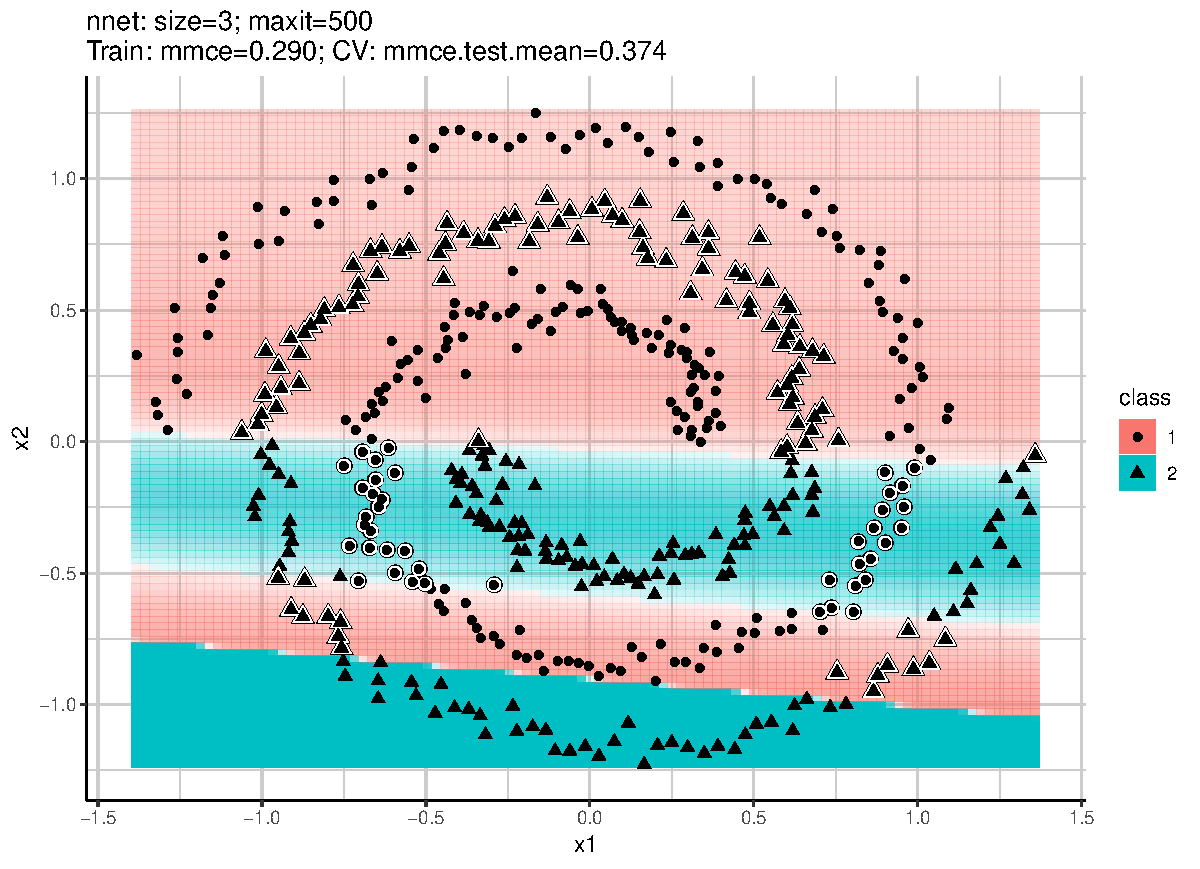
\includegraphics{lab2-solutions_files/figure-latex/unnamed-chunk-6-3.pdf}

\begin{Shaded}
\begin{Highlighting}[]
\FunctionTok{plot\_decision\_boundary\_first\_hidden}\NormalTok{(weights1[}\DecValTok{1}\NormalTok{, }\DecValTok{5}\NormalTok{], weights1[}\DecValTok{2}\NormalTok{, }\DecValTok{5}\NormalTok{], weights1[}\DecValTok{3}\NormalTok{, }\DecValTok{5}\NormalTok{]);}
\end{Highlighting}
\end{Shaded}

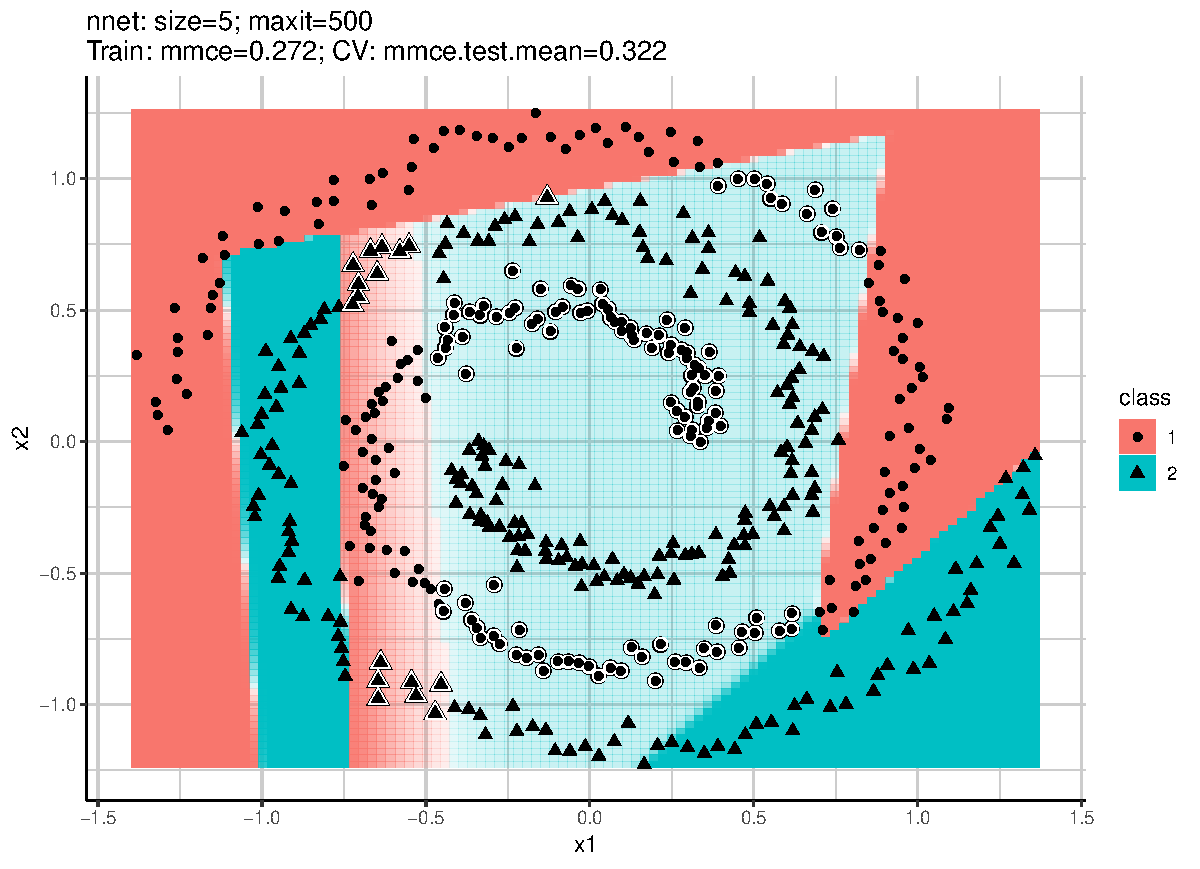
\includegraphics{lab2-solutions_files/figure-latex/unnamed-chunk-6-4.pdf}

And this is the first hidden layer of the network. Let us compute its
predictions for each point of the grid:

\begin{Shaded}
\begin{Highlighting}[]
\NormalTok{hidden1 }\OtherTok{=}\NormalTok{ (}
  \FunctionTok{activation}\NormalTok{(data }\SpecialCharTok{\%*\%}\NormalTok{ weights1)}
\NormalTok{)}

\CommentTok{\# make sure that the number of rows is not changed,}
\FunctionTok{nrow}\NormalTok{(hidden1) }\SpecialCharTok{==} \FunctionTok{nrow}\NormalTok{(data)}
\end{Highlighting}
\end{Shaded}

\begin{verbatim}
## [1] TRUE
\end{verbatim}

\begin{Shaded}
\begin{Highlighting}[]
\CommentTok{\# that there are five columns,}
\FunctionTok{ncol}\NormalTok{(hidden1) }\SpecialCharTok{==} \DecValTok{5}
\end{Highlighting}
\end{Shaded}

\begin{verbatim}
## [1] TRUE
\end{verbatim}

\begin{Shaded}
\begin{Highlighting}[]
\CommentTok{\# and that the values are between zero and one}
\FunctionTok{range}\NormalTok{(hidden1)}
\end{Highlighting}
\end{Shaded}

\begin{verbatim}
## [1] 0 1
\end{verbatim}

\hypertarget{second-hidden-layer}{%
\subsubsection{Second hidden layer}\label{second-hidden-layer}}

The second hidden layer is composed of two neurons, each activating for
inputs inside one of the two triangles that make up our figure. These
two neurons are connected to the four neurons of the previous layer,
thus each of them has five parameters.

Let us first create a new function to visualize the decision boundary of
these neurons in the second hidden layer.

\begin{Shaded}
\begin{Highlighting}[]
\NormalTok{plot\_decision\_boundary\_second\_hidden }\OtherTok{=} \ControlFlowTok{function}\NormalTok{(a, b, c, d, e) \{}
\NormalTok{  neuron\_output }\OtherTok{=}\NormalTok{ (}
    \FunctionTok{activation}\NormalTok{(hidden1 }\SpecialCharTok{\%*\%} \FunctionTok{c}\NormalTok{(a, b, c, d, e))}
\NormalTok{  );}
  \FunctionTok{plot\_grid}\NormalTok{(neuron\_output);}
\NormalTok{\}}

\FunctionTok{plot\_decision\_boundary\_second\_hidden}\NormalTok{(}\SpecialCharTok{{-}}\DecValTok{2}\NormalTok{, }\DecValTok{3}\NormalTok{, }\SpecialCharTok{{-}}\DecValTok{1}\NormalTok{, }\SpecialCharTok{{-}}\DecValTok{3}\NormalTok{, }\DecValTok{1}\NormalTok{);}
\end{Highlighting}
\end{Shaded}

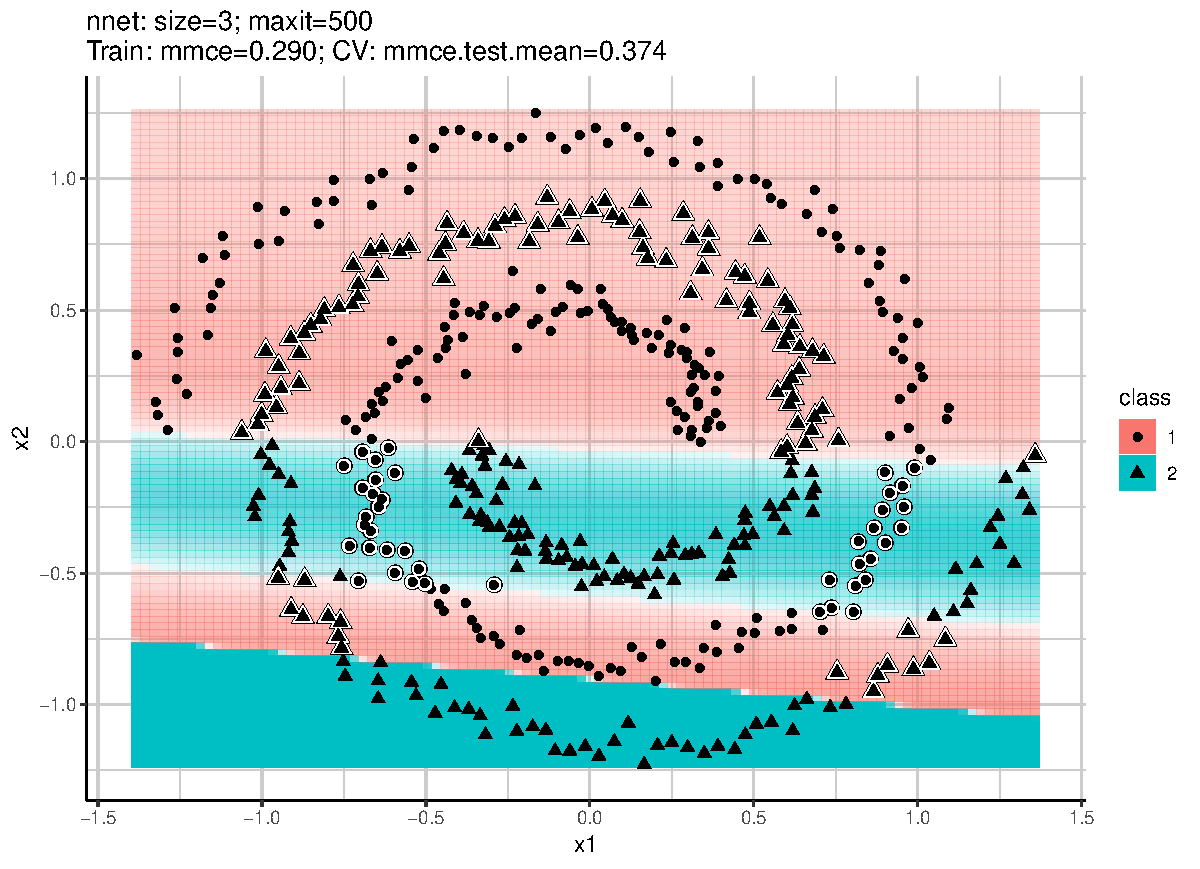
\includegraphics{lab2-solutions_files/figure-latex/unnamed-chunk-8-1.pdf}

Now, as before, find the coefficients for the two neurons and put them
into a matrix with five rows and three columns. You can use the previous
function to help you find these weights.

\textbf{Hint:} you can think of these neurons as performing a logical
AND operation on the outputs of the neurons of the previous layer. All
points inside each triangle must be on the same side of three decision
boundaries.

\begin{Shaded}
\begin{Highlighting}[]
\NormalTok{weights2 }\OtherTok{=} \FunctionTok{matrix}\NormalTok{(}\FunctionTok{c}\NormalTok{(}
  \DecValTok{1}\NormalTok{, }\DecValTok{0}\NormalTok{, }\DecValTok{0}\NormalTok{, }\DecValTok{0}\NormalTok{, }\DecValTok{0}\NormalTok{,  }\CommentTok{\# bias neuron connected to the bias of the previous layer}
  \SpecialCharTok{{-}}\DecValTok{5}\NormalTok{, }\DecValTok{2}\NormalTok{, }\DecValTok{0}\NormalTok{, }\DecValTok{2}\NormalTok{, }\DecValTok{2}\NormalTok{,}
  \SpecialCharTok{{-}}\DecValTok{1}\NormalTok{, }\DecValTok{0}\NormalTok{, }\DecValTok{2}\NormalTok{, }\SpecialCharTok{{-}}\DecValTok{2}\NormalTok{, }\SpecialCharTok{{-}}\DecValTok{2}
\NormalTok{), }\AttributeTok{ncol =} \DecValTok{3}\NormalTok{)}

\FunctionTok{dim}\NormalTok{(weights2)}
\end{Highlighting}
\end{Shaded}

\begin{verbatim}
## [1] 5 3
\end{verbatim}

The predictions:

\begin{Shaded}
\begin{Highlighting}[]
\FunctionTok{plot\_decision\_boundary\_second\_hidden}\NormalTok{(}
\NormalTok{  weights2[}\DecValTok{1}\NormalTok{, }\DecValTok{2}\NormalTok{], weights2[}\DecValTok{2}\NormalTok{, }\DecValTok{2}\NormalTok{], weights2[}\DecValTok{3}\NormalTok{, }\DecValTok{2}\NormalTok{], weights2[}\DecValTok{4}\NormalTok{, }\DecValTok{2}\NormalTok{], weights2[}\DecValTok{5}\NormalTok{, }\DecValTok{2}\NormalTok{]}
\NormalTok{);}
\end{Highlighting}
\end{Shaded}

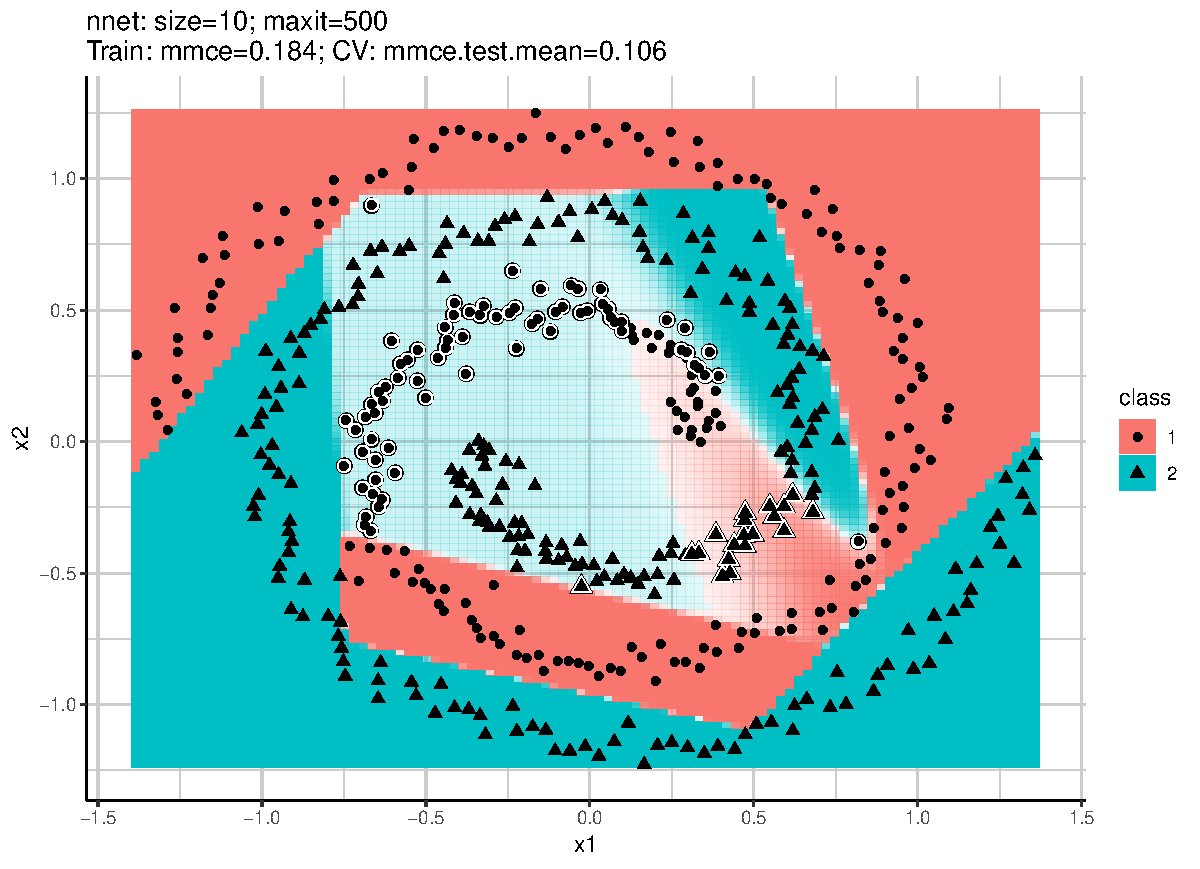
\includegraphics{lab2-solutions_files/figure-latex/unnamed-chunk-10-1.pdf}

\begin{Shaded}
\begin{Highlighting}[]
\FunctionTok{plot\_decision\_boundary\_second\_hidden}\NormalTok{(}
\NormalTok{  weights2[}\DecValTok{1}\NormalTok{, }\DecValTok{3}\NormalTok{], weights2[}\DecValTok{2}\NormalTok{, }\DecValTok{3}\NormalTok{], weights2[}\DecValTok{3}\NormalTok{, }\DecValTok{3}\NormalTok{], weights2[}\DecValTok{4}\NormalTok{, }\DecValTok{3}\NormalTok{], weights2[}\DecValTok{5}\NormalTok{, }\DecValTok{3}\NormalTok{]}
\NormalTok{);}
\end{Highlighting}
\end{Shaded}

\includegraphics{lab2-solutions_files/figure-latex/unnamed-chunk-10-2.pdf}

\begin{Shaded}
\begin{Highlighting}[]
\NormalTok{hidden2 }\OtherTok{=}\NormalTok{ (}
  \FunctionTok{activation}\NormalTok{(hidden1 }\SpecialCharTok{\%*\%}\NormalTok{ weights2)}
\NormalTok{)}

\CommentTok{\# make sure that the number of rows is not changed,}
\FunctionTok{nrow}\NormalTok{(hidden2) }\SpecialCharTok{==} \FunctionTok{nrow}\NormalTok{(data)}
\end{Highlighting}
\end{Shaded}

\begin{verbatim}
## [1] TRUE
\end{verbatim}

\begin{Shaded}
\begin{Highlighting}[]
\CommentTok{\# that there are three columns,}
\FunctionTok{ncol}\NormalTok{(hidden2) }\SpecialCharTok{==} \DecValTok{3}
\end{Highlighting}
\end{Shaded}

\begin{verbatim}
## [1] TRUE
\end{verbatim}

\begin{Shaded}
\begin{Highlighting}[]
\CommentTok{\# and that the values are between zero and one}
\FunctionTok{range}\NormalTok{(hidden2)}
\end{Highlighting}
\end{Shaded}

\begin{verbatim}
## [1] 0 1
\end{verbatim}

\hypertarget{output-layer}{%
\subsubsection{Output layer}\label{output-layer}}

Finally, we can seek the parameters for the output neuron. It should
activate when an input is inside either one of the two triangles.

\textbf{Hint:} you can think of the output neuron as performing a
logical OR operation on the outputs of the second hidden layer.

Let us again modify the visualization function to show the decision of
the network:

\begin{Shaded}
\begin{Highlighting}[]
\NormalTok{plot\_decision\_boundary\_output }\OtherTok{=} \ControlFlowTok{function}\NormalTok{(a, b, c) \{}
\NormalTok{  neuron\_output }\OtherTok{=}\NormalTok{ (}
\NormalTok{    hidden2 }\SpecialCharTok{\%*\%} \FunctionTok{c}\NormalTok{(a, b, c)}
\NormalTok{  );}
  \FunctionTok{plot\_grid}\NormalTok{(neuron\_output);}
\NormalTok{\}}
\end{Highlighting}
\end{Shaded}

Now fill in the parameters:

\begin{Shaded}
\begin{Highlighting}[]
\NormalTok{weights3 }\OtherTok{=} \FunctionTok{matrix}\NormalTok{(}\FunctionTok{c}\NormalTok{(}
  \CommentTok{\# no bias neuron this time}
  \DecValTok{0}\NormalTok{, }\DecValTok{1}\NormalTok{, }\DecValTok{1}
\NormalTok{), }\AttributeTok{ncol =} \DecValTok{1}\NormalTok{)}

\FunctionTok{dim}\NormalTok{(weights3)}
\end{Highlighting}
\end{Shaded}

\begin{verbatim}
## [1] 3 1
\end{verbatim}

The output of the neural network is:

\begin{Shaded}
\begin{Highlighting}[]
\FunctionTok{plot\_decision\_boundary\_output}\NormalTok{(weights3[}\DecValTok{1}\NormalTok{, }\DecValTok{1}\NormalTok{], weights3[}\DecValTok{2}\NormalTok{, }\DecValTok{1}\NormalTok{], weights3[}\DecValTok{3}\NormalTok{, }\DecValTok{1}\NormalTok{]);}
\end{Highlighting}
\end{Shaded}

\includegraphics{lab2-solutions_files/figure-latex/unnamed-chunk-14-1.pdf}

Let us recap how the output is computed:

\begin{Shaded}
\begin{Highlighting}[]
\NormalTok{hidden1 }\OtherTok{=} \FunctionTok{activation}\NormalTok{(data }\SpecialCharTok{\%*\%}\NormalTok{ weights1)}
\NormalTok{hidden2 }\OtherTok{=} \FunctionTok{activation}\NormalTok{(hidden1 }\SpecialCharTok{\%*\%}\NormalTok{ weights2)}
\NormalTok{output }\OtherTok{=}\NormalTok{ hidden2 }\SpecialCharTok{\%*\%}\NormalTok{ weights3}
\end{Highlighting}
\end{Shaded}

This is, in essence, the \emph{forward pass}.

If you did everything correctly, you should see below the bow tie image
we wanted to reproduce:

\begin{Shaded}
\begin{Highlighting}[]
\FunctionTok{plot\_grid}\NormalTok{(output)}
\end{Highlighting}
\end{Shaded}

\includegraphics{lab2-solutions_files/figure-latex/unnamed-chunk-16-1.pdf}

\hypertarget{exercise-3}{%
\subsection{Exercise 3}\label{exercise-3}}

\textbf{Note:} Focus on solving the second exercise first, as this
exercise is of secondary importance. Essentially, it shows that the same
function can be computed by many different neural networks.

Consider a neuron with incoming weights \(\textbf{w}=w_1,\ldots,w_n\)
bias \(b\), and activation \(\tau(\cdot)\). This neuron is connected to
the \(i\)-th neuron of the next layer with the weight \(v_i\), and the
bias of the latter neuron is \(c_i\). We want to replace \(\textbf{w}\),
\(v_i\), \(b\) and \(c_i\) with new parameters \(\textbf{w}'\),
\(v'_i\), \(b'\) and \(c'_i\) so that the output of the network is
unchanged for all inputs. At least one of the new parameters must be
different, but some are allowed to equal the old ones.

\begin{enumerate}
\def\labelenumi{\arabic{enumi}.}
\tightlist
\item
  Suppose that \(\tau\) is the hyperbolic tangent. Show that the network
  computes the same function if we let \(\textbf{w}'=-\textbf{w}\),
  \(v'_i=-v_i\), \(b'=-b\) and \(c'_i=c_i\).
\item
  Now suppose that \(\tau\) is the logistic sigmoid function. How should
  you set \(\textbf{w}'\), \(v'_i\), \(b'\) and \(c'_i\)? Hint: first,
  find the relationship between \(\sigma(x)\) and \(\sigma(-x)\).
\item
  Can you find other ways of modifying the parameters of a neural
  network without altering its output? Equivalently, given a neural
  network computing a certain function, how can you find a different
  network that computes the same function?

  \begin{itemize}
  \tightlist
  \item
    You do not have to provide a formal answer, but you can do so if you
    wish.
  \end{itemize}
\end{enumerate}

\hypertarget{solution-1}{%
\subsubsection{Solution}\label{solution-1}}

\begin{enumerate}
\def\labelenumi{\arabic{enumi}.}
\item
  The output of the neuron is
  \(z'=\tanh(\textbf{w}'^T\textbf{x}+b')=\tanh(-\textbf{w}^T\textbf{x}-b)\).
  Since \(\tanh(x)=-\tanh(-x)\), we have
  \(z'=-\tanh(\textbf{w}^T\textbf{x}+b)=-z\). Since \(v'_i=-v_i\), we
  have that \(v'_iz'=(-v_i)\cdot(-z)=v_iz\). Therefore, no change to
  \(c_i\) is necessary.
\item
  We first prove that \(\sigma(x)=1-\sigma(-x)\):

  \begin{align*}
  \sigma(x)-1+\sigma(-x)
  &=\frac{1}{1+e^{-x}}-1+\frac{1}{1+e^x} \\
  &=\frac{(1+e^x)-(1+e^{-x})(1+e^{x})+(1+e^{-x})}{(1+e^{-x})(1+e^{x})} \\
  &=\frac{1+e^x-1-e^x-e^{-x}-e^0+1+e^{-x}}{(1+e^{-x})(1+e^{x})} \\
  &=0
  \end{align*}

  We can follow the same idea as the previous question, and set
  \(\textbf{w}'=-\textbf{w}\), \(v_i'=-v_i\) and \(b'=-b\). Then, we
  have
  \(z'=\sigma(\textbf{w}'^T\textbf{x}+b')=\sigma(-\textbf{w}^T\textbf{x}-b')=1-\sigma(\textbf{w}^T\textbf{x}+b)=1-z\).
  Since \(v'_i=-v_i\), the contribution of this neuron to the neurons of
  the next layer is \(v'_iz'=-v_i(1-z)=-v_i+v_iz\), therefore we can set
  \(c_i'=c_i+v_i\).
\end{enumerate}

\end{document}
